The following chapter will describe the software that was implemented as part of this thesis. The software is supposed to read in an \gls{bpmn}2.0 Diagram and return a set of suggestions how this BPMN can be improved according to the best-practices described in the first chapters.

This chapter will start with describing the technical implementation and used technologies that were used as well as details on how the software is structured and how it can be used. 
Moreover, this chapter will describe the REST-interface that was implemented and Objects returned by the software. 

Finally the suggestions that can be made to an executable BPMN will be described in section \ref{last}. Some of this suggestions will not be suitable to automation. Explanations on why certain suggestions where implemented and others not will also be provided in this section.
\section{Software Architecture}
The Software was implemented as an Spring Boot Server\cite{spring-boot} Application. The software was developed using git\cite{git} as version control system and the git project is available as an open source project on \url{https://github.com/dsunaric/epms-service}.\\~\\

This software is implemented using maven\cite{maven} as a build-tool, therefore software artifacts can be added to the local repository using the command \verb|mvn install|. This also generates the API sources into the \verb|target| directory. After that the packaged .jar file can be run using the command \verb|java -jar target/*.jar|. 


\subsection{BPMN Processing}
For reading in and processing the BPMN models the Camunda-Model-API\cite{camunda-model-api} was used. The reason for that was the detailed documentation and better usability compared to using an XML parser. The Camunda Model API is able to process most BPMN 2.0 elements. A list of supported elements can be found in the \textit{instance} package\cite{camunda-model-api-spoorted-elements}.
% BPMN 2.0
% cmaunda BPMN model API
\subsection{Folder structure}~\\
The following visualizes and describes the important parts of the projects folder structure:
\dirtree{%
	.1 epms-service.
	.2 src.
		.3 main.
			.4 java.
				.5 at.
					.6 epms.
						.7 api\DTcomment{contains implemented API}.
						.7 entity.
						.7 mapper.
						.7 service\DTcomment{contains suggestion logic}.
							.8 validator\DTcomment{contains validators for the specified best-practices}.
			.4 resources.
				.5 api\DTcomment{contains API specification}.
				.5 config\DTcomment{contains Spring Boot configuration}.
			.4 webapp\DTcomment{contains generated sources for potential clients}.
	.2 target\DTcomment{contains executable .jar file after build} .
}

\section{Interface}
The API was designed and developed using OpenAPI and Swagger\cite{swagger}. The OpenAPI definition is written in one \textit{.yaml} file which is located in the folder\\ \verb|epms-service/src/main/resources/api|.

After Starting the Software, the API description is accessible on \\ \verb|localhost:8080/documentation/v3/api-docs| and can directly be used for code generation by potential frontend applications. 

The application has only one REST-Endpoint, \verb|GET /suggestions|. This endpoint has the process model as request body and returns a list of \textbf{AppliedRules} Objects. 

One \textbf{AppliedRule} object has the following attributes:
\begin{itemize}
	\item \textbf{title}: The title of the applied Rule
	\item \textbf{description}: The description of the rule. Explains when the Rule applies.
	\item \textbf{details}: Explains details about the rule and gives explanation about the effected elements.
	\item \textbf{effectedElements}: A list of elements that violate this rule. The id, name and type (event or task) of the effected element is returned.
\end{itemize} 
\section{Suggestions for improvement}\label{last}
This section describes a set of possible suggestions for improving a BPMN Model. Not all of those rules where implemented as some are not suitable for automation or would be beyond the scope of this thesis. 

\subsection{Comply with Naming Conventions}
BPMN models, no matter if conceptual or executable, should meet naming conventions as it is described in section \ref{naming}. One aspect of naming conventions is the recommended maximum length of five words for any label. 

Since natural language processing would go beyond the scope of this thesis and naming conventions apply to not only executable BPMN, this suggestion for improvement was not fully automated in the context of this thesis. Because of its simplicity, suggesting to rename a element when the label is too long (greater than five words) was implemented.

\subsection{Extend automation boundaries}
The first step of turning an conceptual process model executable is identifying the automation boundaries \ref{automation}. In order to optimize na existing process one could think of extending those existing boundaries and brainstorming ideas to automatize tasks that are not yet automatable. 

This requires a lot of domain specific knowledge and can therefore not be simply implemented.

\subsection{Eliminate Manual Tasks}
As describes in section \ref{manual} Manual Tasks should not be part of an executable BPMN diagram and should if possible be automated using service tasks or, if that is not possible, be replaced by user tasks. 

Manual tasks are identified by the software. The returned effected elements represent a list of manual tasks in the given diagram.

\subsection{Complete the process model}
Another manual step to improve a process model, is making sure the process model is complete section \ref{complete}.

Since this would also require domain specific knowledge, the software does not include analyzing the process model for incompleteness.

\subsection{No two consecutive Tasks handled by the same resource}
Two task that are executed one after the other should be merged, if they have the same enitity executing the task. As described in section \ref{granulartity}, bringing the model to an adequate granularity level minimizes handovers and overhead. In case of User tasks this means the same usergroup is executing both tasks. Automated Tasks that follow each other should also always be merged to minimize flownodes.


The software recognizes such consective tasks return a list of effected elements that represent the tasks that can be merged with its direct successor. In case that three or more tasks can be merged, this algorithm will return every task that can be merged with its successor on its own. Therefore if ``task1`` , ``task2`` and ``task3`` can be merged all together, the algorithm will return ``task2`` and ``task3`` as effected elements.

An example on when this rule is satisfied can be found in figure \ref{fig:example-EX}. The software will return \textit{Task A}, \text{Task B} and \textit{Task D} as effected elements, indicating, that  \textit{Task D} should be merged with its successor ( \textit{Task E}),  \textit{Task A} should be merged with  \textit{Task C} and  \textit{Task B} should be merged with  \textit{Task C}, therefore merging all three Tasks ( \textit{Task A}, \textit{Task B} and  \textit{Task C})together. An example for an resulting process model, after this suggestions are applied, can be found in figure \ref{fig:example-EX-fix}.

\begin{figure}[H]
	\centering
	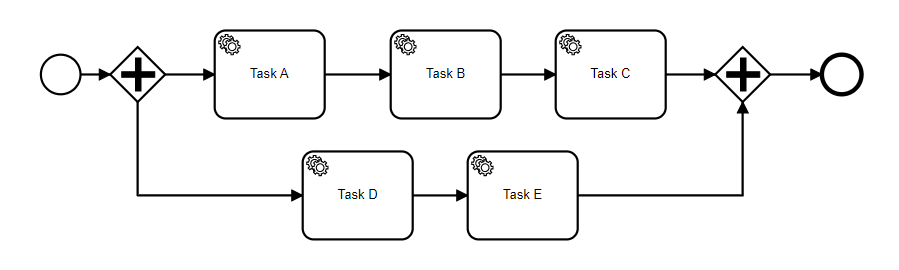
\includegraphics[width=0.9\columnwidth]{graphics/merge-suggestion-1}
	\caption{Example of a process where tasks can be merged together} 
	\label{fig:example-EX} 
\end{figure}

\begin{figure}[H]
	\centering
	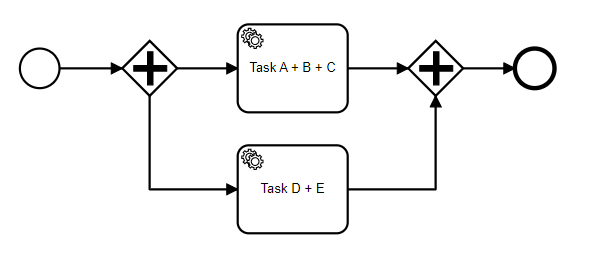
\includegraphics[width=0.7\columnwidth]{graphics/merge-suggestion-2}
	\caption{change necessary for the process in \ref{fig:example-EX} so satisfy this rule} 
	\label{fig:example-EX-fix} 
\end{figure}

\subsection{Inclusive Gateways over combining parallel and exclusive Gateways}
In order to save flownodes, inclusive gateways should be used instead of a parallel gateway followed by one or more exclusive gateways. An example for this kind of pattern is shown in \ref{fig:example-GW}.

\begin{figure}[H]
	\centering
	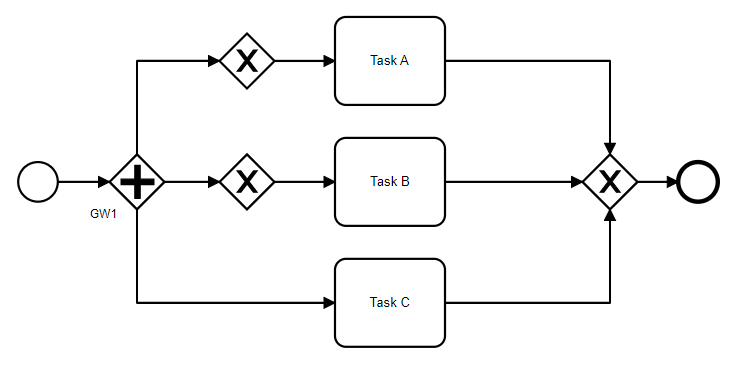
\includegraphics[width=0.9\columnwidth]{graphics/exclusive-suggestion-1}
	\caption{Example for a parallel gateway followed by one or more exclusive gateways} 
	\label{fig:example-GW} 
\end{figure}

The software applies this rule whenever a parallel gateways is followed by one or more exclusive gateways. The returned effected elements are a list of parallel gateways that are followed by one or more exclusive gateways in the given diagram. In the example shown in  \ref{fig:example-GW}, the returned element would be \textit{GW1} and the change to comply with this rule would be shown in \ref{fig:example-GW-fix}
\begin{figure}[H]
	\centering
	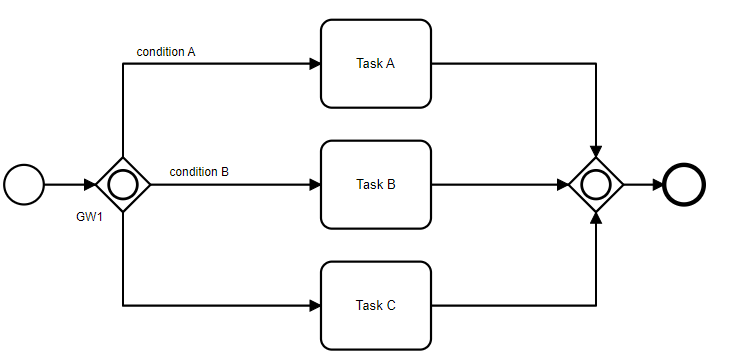
\includegraphics[width=0.9\columnwidth]{graphics/exclusive-suggestion-2}
	\caption{change necessary for the process in \ref{fig:example-GW} so satisfy this rule} 
	\label{fig:example-GW-fix} 
\end{figure}

\subsection{Value Added Analysis}
In order to eliminate tasks in a process that have limited value for the customer, a value added analysis as explained in section \ref{vaa} can be performed.  

This would also require domain specific knowledge and is therefore not done by the software. 

\subsection{Evaluate Suggestions Quantitative}

Finally, all process models as a result of applying any of those suggestions made by the software or manually, can be evaluated against each other using quantitative measures. The section \ref{quant} describes approaches to estimating quantitative measures using flow analysis. 

Since BPMN 2.0 has no option to integrate estimations for quantitative measures for processes or tasks, and estimation would require detailed knowledge about the process at hand, this will not be implemented.